\chapter{Examples}
\label{ch:04}

Preface (optional, remove from \texttt{\textbackslash includeonly} in \texttt{main.tex} if wanted). To reference a section, e.g. the literature review you can use \texttt{\textbackslash cref\{labelName\}} to reference it as \cref{ch:lit-review}. 

\enquote{This is an \enquote{inner quote} inside an outer quote}, according to the specified language's typesetting.

\vspace{\baselineskip}
\noindent
Skipping a line and dropping the indent can be used in addition to indents by using \\ \texttt{\textbackslash vspace\{\textbackslash baselineskip\}} \texttt{\textbackslash noindent} when natural.




\section{Sections can be used}
With section text. Above sections are chapters, and above that again are parts (add those in \texttt{main.tex}).

\subsection{And subsections}

\subsubsection{And subsubsections}
The subsubsection text can start right after a subsection for example.

\paragraph{And paragraphs}
Paragraphs are on the level below subsubsections.


\subparagraph{There is also subparagraphs} In summary, see \cref{tab:levels}.
\begin{table}[H]
    %\centering     % handbook says not to center!
    \caption{Memoir document class levels.}
    \begin{tabularx}{1\textwidth}{l|X}
        \textbf{Name} & \textbf{Note} \\ \hline
        Part & Add in \texttt{main.tex} \\
        Chapter & Each chapter is located under the folder \texttt{Chapters}, remember to include them in \texttt{main.tex} (in both places)! \\
        Section & \\
        Subsection & To turn of numbering and/or remove subsections from ToC, edit the preamble (search for documentclass levels). \\
        Subsubsection & \\
        Paragraph & \\
        Subparagraph & \\
    \end{tabularx}
    \label{tab:levels}
\end{table}

\LaTeX{} tables can be very compact, so the above table can easily be altered by wrapping the following around it (and the values can be changed for more or less spacing, independently):
\begin{minted}{latex}
\setlength{\tabcolsep}{0.5em}       % for the horizontal padding
{\renewcommand{\arraystretch}{1.5}  % for the vertical padding
% Table code here!
}
\end{minted}

\setlength{\tabcolsep}{0.5em}       % for the horizontal padding
{\renewcommand{\arraystretch}{1.5}  % for the vertical padding
\begin{table}[H]
    %\centering     % handbook says not to center!
    \caption{Memoir document class levels, with more spacing.}
    \begin{tabularx}{1\textwidth}{l|X}
        \textbf{Name} & \textbf{Note} \\ \hline
        Part & Add in \texttt{main.tex} \\
        Chapter & Each chapter is located under the folder \texttt{Chapters}, remember to include them in \texttt{main.tex} (in both places)! \\
        Section & \\
        Subsection & To turn of numbering and/or remove subsections from ToC, edit the preamble (search for documentclass levels). \\
        Subsubsection & \\
        Paragraph & \\
        Subparagraph & \\
    \end{tabularx}
    \label{tab:levels-space}
\end{table}
}

Also shown above, the package \texttt{minted} can also be used to display code snippets, e.g. Python code:
\begin{minted}{python}
import numpy as np

# Generate 2x3 uniformly random numbers between -1 and 1:
random_array = np.random.uniform(low=-1.0, high=1.0, size=(2,3))
\end{minted}
Note         that everything inside the \texttt{minted} environment is space sensitive, unlike       \LaTeX{} code in         general.

\subsection{Figures}
\cref{fig:logo} is an example of how to import and scale the size of figures or images, to e.g. 52 \% of the textwidth. If not required to left justify figure captions, edit the preamble (search for \enquote{captions}). Remember to add alternative text (alt text) for accessibility – a brief description of the figure for readers with visual impairments – as required in the handbook!

\begin{minted}{latex}
\begin{figure}[H]
    %\centering     % handbook says not to center!
    \includegraphics[width=0.52\textwidth, alt={Alt text here}]{figure-file.png}
    \caption{Figure caption}
    \label{fig:figure-label}
\end{figure}   
\end{minted}

\begin{figure}[H]
    %\centering     % handbook says not to center!
    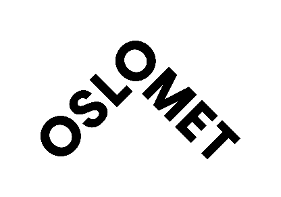
\includegraphics[width=0.52\textwidth, alt={Oslo Metropolitan University's logo, in black on white.}]{oslomet_logo.png}
    \caption{Oslo Metropolitan University's logo.}
    \label{fig:logo}
\end{figure}



\section{For titles with \texorpdfstring{e.g. \(\R^3\)  or \LaTeX{}}{LaTeX code}}

For any titles with \LaTeX{} code (e.g. math mode), use the following macro provided by the \texttt{hyperref} package to provide a text-only version of the title as well: \\
\begin{minted}{latex}
    \texorpdfstring{<latex-code>}{<bookmark-text>}
\end{minted}

\vspace{\baselineskip} \noindent
This can also be seen in the abstract title, where \LaTeX{} code was used to make it centred in the displayed version:
\begin{minted}{latex}
    \chapter{\texorpdfstring{\centering Abstract}{Abstract}}
\end{minted}

\subsection{Rigid body motions in \texorpdfstring{\(\R^3\)}{real three dimensional space}}
An example how how this might be used is this title, given by
\begin{minted}{latex}
\subsection{Rigid body motions in \texorpdfstring{\(\R^3\)}{real 3-dimensional space}}
\end{minted}
